\documentclass[../main.tex]{subfiles}

\begin{document}
\chapter{Numerical Results}
\label{chap:results}
In this chapter, I will go give an overview of the numerical implementation of the cross-sections from the earlier chapters.
This is an entirely non-trivial process, and I use multiple external packages to do the calculations.
Particularly, the numerical integration over the PDFs requires a good deal of finesse.
The algorithm used for the integration is the \verb|VEGAS| algorithm~\cite{Vegas1}, implemented in \verb|C++| in the GNU Scientific Library (\verb|GSL|)~\cite{GSL}.
The values for the PDFs at a given energy scale \(\mu\), along with values for \(\alpha_s\), are taken from the \verb|LHAPDF| package~\cite{LHAPDF}.
MSSM and CMSSM particle spectra are generated in SLHA file format using \verb|FlexibleSUSY|~\cite{FlexibleSUSY1,FlexibleSUSY2}.
To evaluate the Passarino-Veltman loop integrals, I use the package \verb|LoopTools|~\cite{LoopTools}.
\medskip

The numerical results presented in this chapter are meant to showcase the possibility of parameter space exploration of the full MSSM Lagrangian for the cross-sections calculated in this thesis.
To this end, only the expressions for neutralino pair production have been implemented, and will be the focus of this chapter.
A proper analysis of the MSSM parameter space as it pertains to electroweakino production, and comparison to experiment at the LHC, is beyond the scope of this thesis.

The implementation of the cross-sections in this thesis have been done in \verb|C++| in the currently unpublished codebase \verb|smoking|~\cite{smoking}.



\section{Setup and Execution}
There are a few things that go into setting up and performing the computation of a full cross-section given an MSSM parameter point -- I will go briefly over some of these details here.
All results are computed with a centre-of-mass energy for the proton collisions set to \(\sqrt{S} = 13.6\,\text{GeV}\) to match the LHC run 3.

\subsection{Renormalisation Scheme}
\label{res:subsec:renormalisation_scheme}
Throughout the thesis, I have mentioned the renormalisation schemes that will be used, but I will take a moment to summarise them here.
Masses of all particles are renormalised in the on-shell scheme, as has already been performed for the quarks in \cref{pc:subsec:counterterms}.
Later in this section, I will go through our usage of the spectrum calculator \verb|FlexibleSUSY|, which calculates on-shell renormalised masses for sparticles given an MSSM parameter point.
The strong coupling \(\alpha_s\) is renormalised in the \MSbar\ scheme, and its value is calculated at the \emph{renormalisation scale} \(\mu_R\).
The numerical implementation of the running coupling values for \(\alpha_s\) is done in \verb|LHAPDF|, which we also use to evaluate the PDFs.

The scheme for the electromagnetic coupling \(\alpha = \frac{e^2}{4\pi}\) is different, however.
It is related to the parameters of electroweak symmetry breaking, and needs to be renormalised consistently together with these quantities.
In this thesis, I will follow a renormalisation scheme for the electroweak parameters as utilised in~\cite{Denner:2019vbn}, named the \(G_\mu\)-scheme.
From the weak coupling \(g\), the hypercharge coupling \(g^\prime\) and the Higgs vacuum expectation value \(v\), we have the relations between the parameters of the electroweak sector after symmetry breaking
\begin{subequations}
  \begin{eqnarray}
    m_W &=& \frac{1}{2}v g, \\
    m_Z &=& \frac{1}{2} v \sqrt{g^2 + g^{\prime 2}}, \\
    e &=& \frac{g g^\prime}{\sqrt{g^2 + g^{\prime 2}}}, \\
    \sin\theta_W &=& \frac{g^\prime}{\sqrt{g^2 + g^{\prime 2}}}.
  \end{eqnarray}
\end{subequations}
Keeping the same convention as \verb|Resummino|~\cite{Resummino}, we will renormalise the \(W\)- and \(Z\)-boson masses in the on-shell scheme and the coupling strength and vacuum expectation value be fixed by the Fermi constant \(G_F \approx 1.16638 \times 10^{-5} \text{GeV}^{-2}\).
This fixes the Weinberg angle and the fine-structure constant by
\begin{subequations}
  \begin{eqnarray}
    \sin^2\theta_W &=& 1 - \frac{m_W^2}{m_Z^2}, \\
    \alpha &=& \sqrt{2} \frac{G_F m_W^2 \sin^2\theta_W}{\pi}.
  \end{eqnarray}
\end{subequations}
For the \(\alpha_W\) we have used in the calculations thus far, we then have
\begin{equation}
  \alpha_W = \sqrt{2} \frac{G_F m_W^2}{\pi}.
\end{equation}
This last equality shows the independence of the weak coupling we have used on \(\sin\theta_W\), which is a free, running parameter in this scheme.
Thereby, the running of this coupling is actually cancelled to two-loop order, according to~\cite{Denner:2019vbn}, letting us treat \(\alpha_W\) as a constant parameter for our purposes.
There are factors of \(\cos\theta_W\) and \(\sin\theta_W\) that arise in our couplings  in \cref{susy:tab:variable_definitions}, which should receive higher order corrections, but these should be small in the \(G_\mu\)-scheme.
The running of \(\alpha_s\) is significantly larger at these energy scales, and will be the primary source of scale uncertainty in the PDFs and NLO contributions.



\subsection{Uncertainty and Errors}
In the context of collider experiments, where collision data is compared to theoretical simulations using cross-sections such as the ones calculated here, uncertainties are important when statistically comparing predictions from different models.
To make a proper search of the MSSM parameter space, the uncertainty in the theoretical predictions must be taken into account.
These come from various sources; the numerical error from the integration algorithm used, errors in the values of the PDFs at given momentum fractions or factorisation scales, and theoretical uncertainties from truncating the perturbation series before convergence to a `true' value.
Most numerical integration methods have good error estimates, and for somewhat well-behaved functions, these will be adequate.
As it turns out, the numerical precision is not the leading source of error in the calculations we will do here.
PDF errors are usually dealt with by computing the cross-sections for multiple independent PDF sets, and taking sample averages and variances from the cross-sections computed with the different PDFs.
These errors are usually combined with the uncertainty in the strong coupling \(\alpha_s\), as experimentally, it is hard to differentiate the two and determine them accurately individually.
Combined error from PDFs and \(\alpha_s\) determination will be calculated this way using the \verb|PDF4LHC21_40|~\cite{PDF4LHCWorkingGroup:2022cjn} PDF set, with 43 PDF members, indexed \(i = 0, \ldots, 42\).
The first member gives the central value, and the cross-section computed using this member is regarded as the mean cross-section \(\sigma_\text{central}\).
Following the PDF error procedure outlined in~\cite{PDF4LHCWorkingGroup:2022cjn}, we compute the PDF error \(\delta \sigma_\text{PDF}\) as
\begin{equation}
  \delta\sigma_\text{PDF} = \sqrt{\sum_{i=1}^{42} \pclosed{\sigma(\text{PDF member }i) - \sigma_\text{central}}^2}.
\end{equation}
\medskip

Approximating the uncertainty from higher order corrections to the computation at a finite order is not entirely straight forward.
The procedure we will use is to vary the factorisation and renormalisation scales \(\mu_F\) and \(\mu_R\).
These scales are artificially introduced into the theory, and should drop out of physical predictions of the full perturbation series.
Therefore, we will assume that dependence on these scales should decrease as higher order corrections are taken into account -- essentially meaning that the dependence on these scales is somehow proportional to the uncertainty from the truncation of the perturbation series.
Concretely, we will use the \emph{scale error} as an estimate for the theoretical uncertainty, which we will define by
\begin{subequations}
  \begin{eqnarray}
    \delta\sigma_{\mu}^+ &=& \operatorname{max}(|\sigma(2\mu) - \sigma(\mu)|, |\sigma(2\mu) - \sigma(\mu)|), \\
    \delta\sigma_{\mu}^- &=& \operatorname{min}(|\sigma(2\mu) - \sigma(\mu)|, |\sigma(2\mu) - \sigma(\mu)|),
  \end{eqnarray}
\end{subequations}
where \(\mu\) can either be \(\mu_F\), \(\mu_R\) or both at the same time.
What scale we are varying will be noted where relevant.



\subsection{Spectrum Generation and Scenarios}
Going from the Lagrangian parameters of the MSSM to the mass eigenstates and mixing matrices is a non-trivial transition, as we have already seen when discussing the electroweakino mixing in \cref{susy:sec:electroweakinos,susy:sec:takagi}.
Doing this procedure of spectrum generation makes sure that the renormalised parameters are physically cohesive, rather than what is often done when using simplified models where parameters like particle masses or mixing matrix elements are varied irrespective of their origin in the MSSM Lagrangian.
In the following, I will present the scenarios that we will use for the numerical results in this chapter.

\begin{figure}[ht!]
  \centering
  \begin{subfigure}{\textwidth}
    \centering
    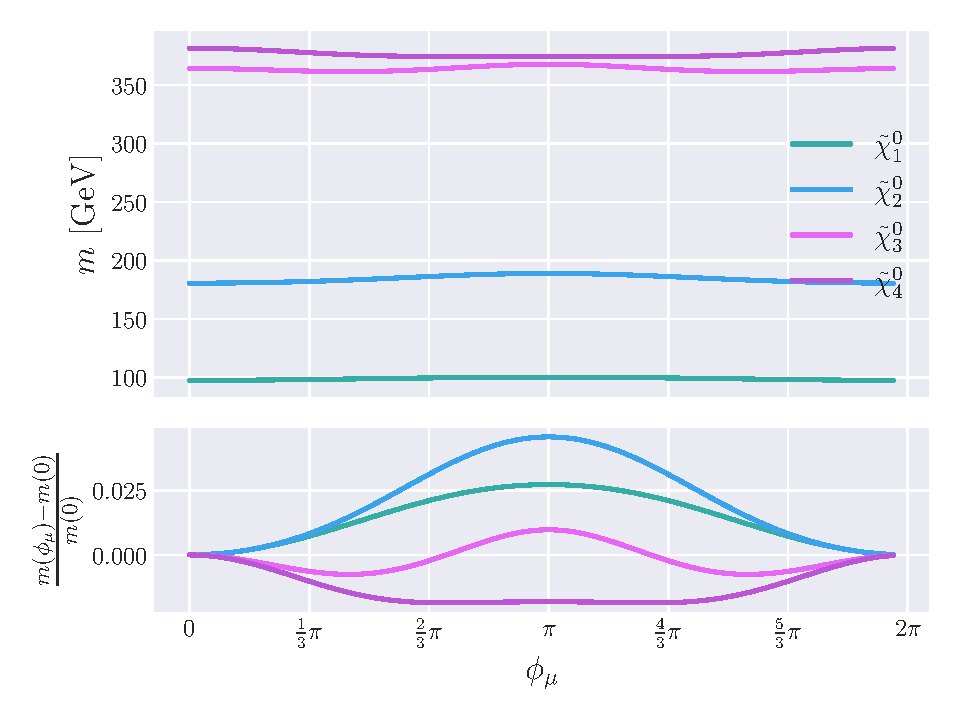
\includegraphics[width=0.85\textwidth]{muCPV/massplot.pdf}
    \caption{}
  \end{subfigure}
  \begin{subfigure}{\textwidth}
    \centering
    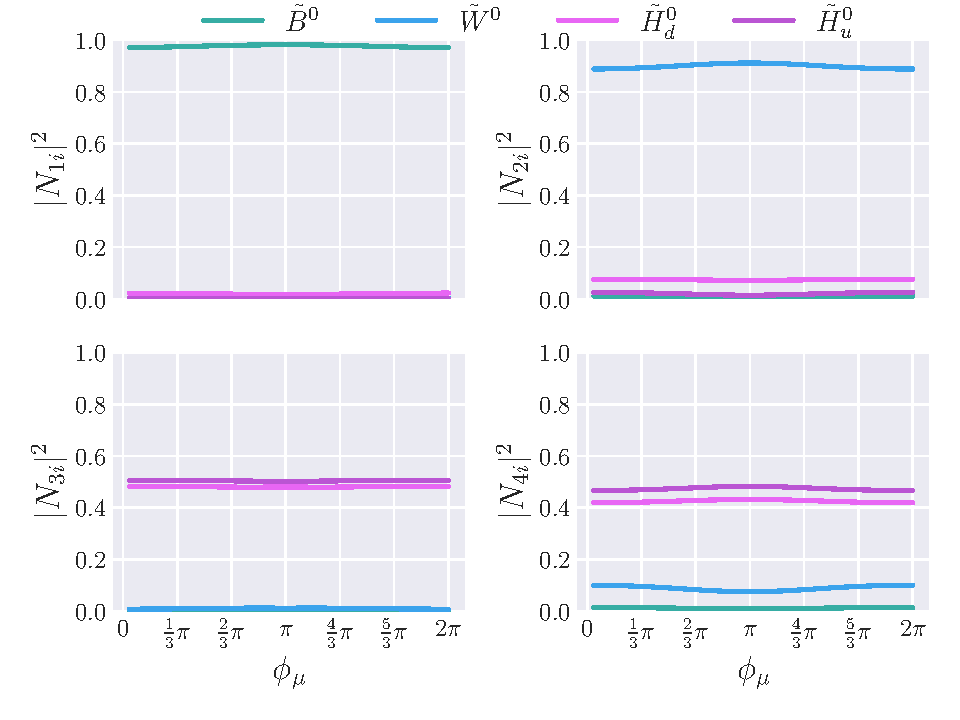
\includegraphics[width=0.85\textwidth]{muCPV/mixplot.pdf}
    \caption{}
  \end{subfigure}
  \caption{A plot showing the neutralino spectrum in the cSPS1a scenario. The first plot shows the neutralino masses as a function of the phase of \(\mu\), whereas the lower plot shows the amount of the interaction eigenstates in each neutralino mass eigenstate. The spectra were generated with \texttt{FlexibleSUSY}.}
  \label{res:fig:csps1a_scenario}
\end{figure}



\subsubsection*{Benchmark Point}
One of the parameter points that I will be using for many of the results is the common benchmark point SPS1a~\cite{sps1a}.
This is based on the mSUGRA~\cite{mSUGRA} model, with the parameters set to
\begin{equation}
  m_0 = 100\,\text{GeV},\quad m_{\sfrac{1}{2}} = 250\,\text{GeV},\quad A_0 = -100\,\text{GeV},\quad \tan\beta = 10,\quad \sgn{\mu} = +.
\end{equation}
Here \(m_0\) is a common soft mass for all the sfermions under the assumptions of no flavour violation, \(m_{\sfrac{1}{2}}\) is a common gaugino mass parameter, \(A_0\) is the common trilinear coupling under the assumption of no flavour mixing and electroweak symmetry breaking is fixed by the SM parameters together with \(\tan\beta = \frac{v_u}{v_d}\) and \(\sgn{\mu}\).
The parameters are taken to be defined at the scale of \(m_{\sfrac{1}{2}} = 250\) GeV, and pole masses and mixing matrices are determined using \verb|FlexibleSUSY| to run the various parameters from this scale.
\medskip

Based on the SPS1a benchmark point, I will explore a variant where the above parameters are allowed to be complex, and the sign of \(\mu\) is replaced by an arbitrary complex phase \(\phi_\mu\).
For future reference, I will refer to this scenario as complex SPS1a (cSPS1a).
This will allow for CP violation in the resulting particle model, and showcases the generality of the calculations from the prior chapters, and implementation thereof.
Particularly, I will explore scenarios where the phase of \(\mu\) is rotated around the complex plane, introducing complex phases in the neutralino mixing matrices, but also slightly complex phases in the squark mixing matrices through the inclusion of loop effects to their mixing matrices.
In fact, loop effects in this scenario also make flavour violating mass terms possible, so the general \(6\by 6\) squark mixing matrices discussed in \cref{susy:sec:feynman_rules} are used.
\medskip

The mass spectrum and mixing of the neutralino sector in the cSPS1a scenario is shown in \cref{res:fig:csps1a_scenario}.
It shows that the lightest neutralino is very bino-like at a mass of \(\sim 100\) GeV, with the next-to-lightest neutralino being wino in nature at around 180 GeV.
The higgsino states mix quite heavily to create two nearly degenerate mass eigenstates at around 375 GeV.
Perhaps surprisingly, the gaugino-like lighter neutralino states are affected the most by the phase of the Higgs mass parameter \(\mu\), relative to the \(\phi_\mu = 0\) case.


\subsubsection*{Higgsino Scenario}
To explore the NLO results that have been calculated, we will need some scenario where two of the neutralino mass eigenstates correspond closely to the pure higgsino states.
This is done by separating \(|\mu|\) from \(|M_1|, |M_2|\), which from a model building perspective is not unnatural, given that no mechanism implies that they should be of the same order of magnitude -- \(\mu\) comes from the supersymmetric part of the Lagrangian, whereas \(M_1, M_2\) as soft masses derived from some supersymmetry breaking mechanism.
Mixing between the higgsino and gaugino states will also be suppressed if \(|M_1|, |M_2| \gg m_Z\), by looking at the non-diagonal terms in \cref{susy:eq:neutralino_mixing_matrix}, so we will choose a scenario with \(|\mu| \ll M_1, M_2\) and \(|\mu| \sim m_Z\).

Such a scenario is significant for electroweakino pair production, as it is mediated by a \(Z\)-boson in the case of neutralino pairs, \(W\)-boson for a neutralino and a chargino, or a \(Z\)-boson and photon for chargino pairs, meaning the cross-sections can become relevant at the centre-of-mass energies at the LHC\@.
This is opposed to the production of gaugino-like neutralinos and charginos, which is mediated through the squarks, which can be much heavier than the electroweak bosons, suppressing the cross-sections.
The notable exception to this is the pair production of gaugino-like charginos, which is also mediated by the \(Z\)-boson and photon.
\medskip

I will choose a scenario with three different scales: A low scale for the higgsino masses \(|\mu| = 100\) GeV, a middle scale for the sfermion and gluino masses at 2000 GeV, and a high scale to decouple the wino and bino mass parameters from the Higgs mass parameter at \(M_{1,2} = 100\) TeV.
These values are all defined at the high scale, which I will call \(M_\text{SUSY} = 100\) TeV, and then run down to get pole masses for the individual particles.
All parameters except the higgsino mass parameter \(\mu\) are taken to be real, whereas the phase of \(\mu\) will be varied.
\medskip
{\renewcommand{\arraystretch}{1.2}
  \begin{table}[ht!]
    \centering
    \begin{tabular}{|r|c|c|c|c|c|c|c|c|}
      \hline
      \textbf{Scenario} & \(|\mu|\) & \(\tan\beta\) & \(M_{1,2}\) & \(M_3\)  & \(m_0\)  & \(M_A\)  & \(A_0\)  & \(M_\text{SUSY}\) \\
      \hline
      Higgsino          & \(100\)   & 10            & \(10^5\)    & \(2000\) & \(2000\) & \(2000\) & \(1000\) & \(10^5\)          \\
      \hline
    \end{tabular}
    \caption{Summary of MSSM parameters defining the Higgsino scenario used in this thesis.
      All parameters except \(\tan\beta\) are given in GeV.
      \(m_0\) denotes the common soft mass for all sfermions, taken to be diagonal in flavour space.
      \(A_0\) is the common soft trilinear coupling, also taken to be diagonal in flavour space.
      A parametrisation of EWSB is chosen where \(M_A\), the mass of the pseudoscalar Higgs boson, is kept as a free parameter.}
  \end{table}
}

Another scenario that will be used for comparison to the LCH SUSY Cross Section Working Group~\cite{SUSYxsecWG} (SXWG) is a simplified Higgsino scenario.
This scenario is an unnatural scenario, meaning masses and mixing angles set `by hand'.
In this scenario the lightest Higgs scalar is set to \(125\) GeV, whereas all other Higgs scalar and sfermion masses are set to \(10^5\) GeV.
The gluino mass, the two largest neutralino masses and the largest chargino mass are all set to \(10^5\) GeV as well, effectively decoupling the supersymmetric particle spectrum except for the higgsinos.
The two lightest neutralinos and lightest chargino are set to be mass degenerate, with a common mass \(m_{\tilde\chi}\) which is varied from 100 GeV to 1500 GeV.
The two higgsino states are set to be maximally mixed.



\section{Comparison}
\label{res:sec:comparison}
To test the verity of our implementation, we first compare to established results.
Particularly, we will compare to results obtained using \verb|Resummino|~\cite{Resummino}.
Two scenarios will be used for comparison:
To compare LO contributions, I will use the SPS1a~\cite{sps1a} benchmark point, and to compare the NLO implementation of the higgsino channel, I will use the simplified model with two, mass degenerate, maximally mixed higgsinos, and the rest of the supersymmetric particle spectrum decoupled described in the previous subsection.
This scenario is taken from~\cite{SUSYxsecWG}.



\subsection{Leading Order Comparison}
To compare the LO implementations, I compare results from the \verb|smoking| implementation to that of \verb|Resummino| in the SPS1a benchmark point.
All neutralino pair production processes are compared, as to make sure the implementation of \(Z\)-boson mediated contribution, squark mediated contribution, and interference between the two, is done correctly.
The results, shown in \cref{res:fig:sps1a_comparison}, exhibit great agreement between the results.
No relative error is above \(0.2\%\), with most staying around \(0.17\%\), which is reasonable up to numerical errors.
However, our results seem to be systematically slightly above those of \verb|Resummino|.
Had the agreement not been as good, this could be investigated further.

\begin{figure}[ht!]
  \centering
  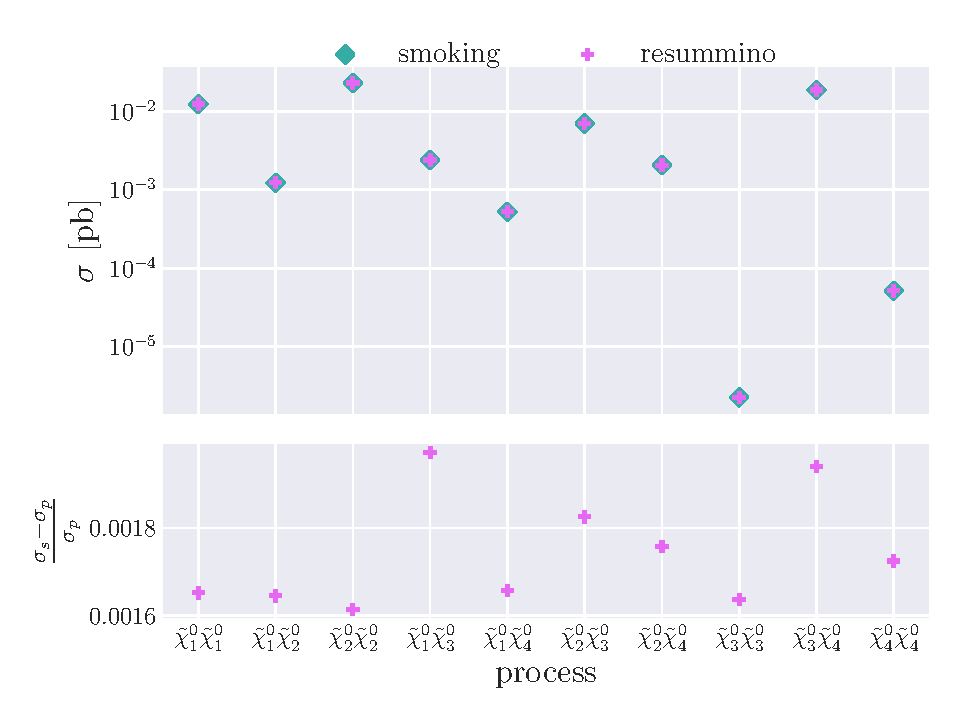
\includegraphics[width=0.85\textwidth]{compare_prospino_sps1a_mod.pdf}
  \caption{Comparison of LO results from this thesis to those from \texttt{Resummino} for all possible neutralino pair processes.
    All cross-sections computed in the SPS1a benchmark point.
    The cross-sections computed with the implementation from this thesis are denoted \(\sigma_s\), whereas results computed with \texttt{Resummino} are denoted \(\sigma_p\).}
  \label{res:fig:sps1a_comparison}
\end{figure}



\subsection{Next-to-Leading Order Comparison}
In \cref{res:fig:hino_comparison} we see a comparison between results computed with \verb|smoking| as compared to \verb|Resummino| and SXWG to NLO\@.
It shows that our results agree with \verb|Resummino| up to a relative error of \(\sim 0.2\%\), and at worst an error of \(\sim 1.5\%\) relative to SXWG at high \(m_{\tilde\chi}\) masses.
Disagreement with \verb|Resummino| is within what can be expected by numerical errors.
Furthermore, there seems not to be systematic overestimation, as could perhaps be seen in \cref{res:fig:csps1a_scenario}.
The discrepancies when comparing to SXWG can be accounted for by the fact that the SXWG results are computed using next-to-leading log (NLL) corrections from the resummation of large logarithms together with the NLO results.
These corrections are indeed not that large, but do become more relevant at higher neutralino masses.
This is because the resummed logarithms give corrections to the soft radiation limit where \(Q^2 \to \hat{s}\).
Since \(Q^2\) is bounded from below by \((m_{\tilde\chi^0_i} + m_{\tilde\chi^0_j})^2\) kinematically, the soft radiation region becomes a larger part of the overall available phase space when the neutralino masses increase.
This shows that the NLL effects in this Higgsino scenario is very small, particularly compared to even LO effects of complexification of the parameters, as we shall see promptly.


\begin{figure}[ht!]
  \centering
  \includegraphics[width=0.85\textwidth]{pure_scenarios/hinoNLO.pdf}
  \caption{Comparison of results from this thesis to those from \texttt{Resummino} and the LHC SUSY Cross Section Working Group.
    Scale error is included in shaded regions around the lines in the upper plot, however, it is so inconsequential as to only be barely visible.}
  \label{res:fig:hino_comparison}
\end{figure}


\section{Scale Dependence and PDF Errors}
In this section, I will explore the errors that go into the cross-section calculations.
Particularly, I will focus on PDF errors and scale errors in the LO and NLO contributions in the Higgsino scenario.
Nonetheless, much of the discussion applies more broadly.

\begin{figure}[ht!]
  \centering
  \begin{subfigure}{0.49\textwidth}
    \centering
    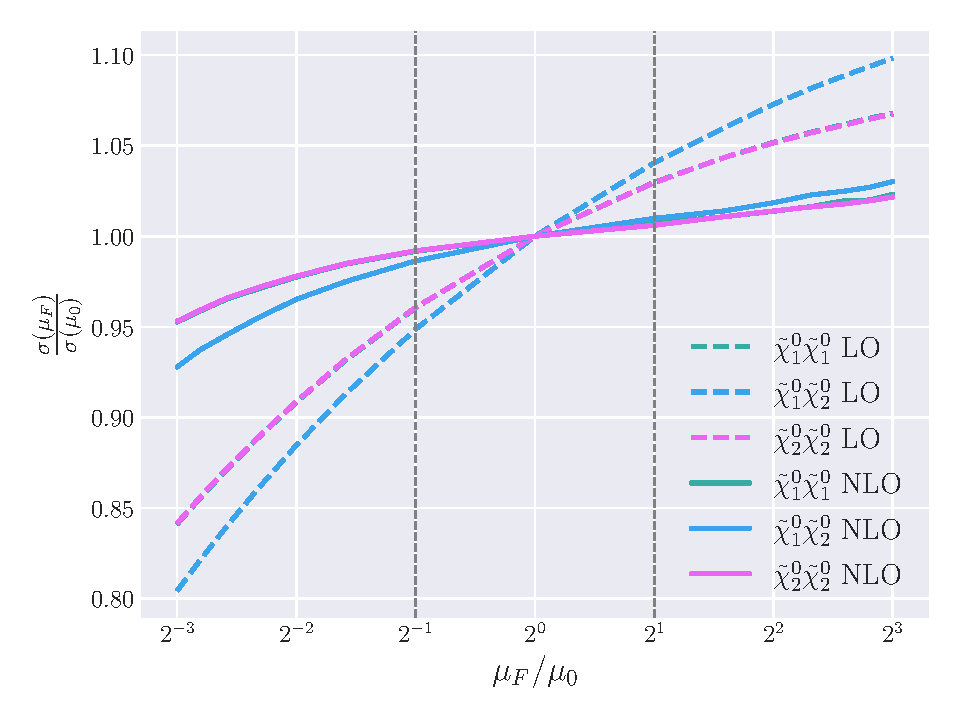
\includegraphics[width=\textwidth]{scaleDependence/mufPlot.pdf}
    \caption{}
  \end{subfigure}
  \begin{subfigure}{0.49\textwidth}
    \centering
    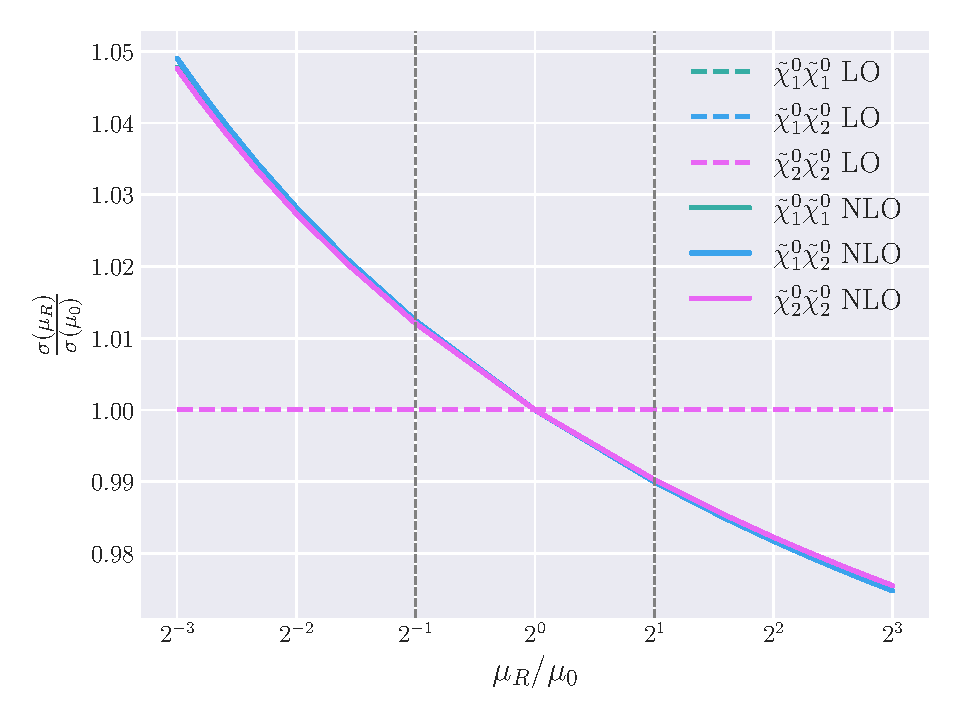
\includegraphics[width=\textwidth]{scaleDependence/murPlot.pdf}
    \caption{}
  \end{subfigure}
  \begin{subfigure}{0.49\textwidth}
    \centering
    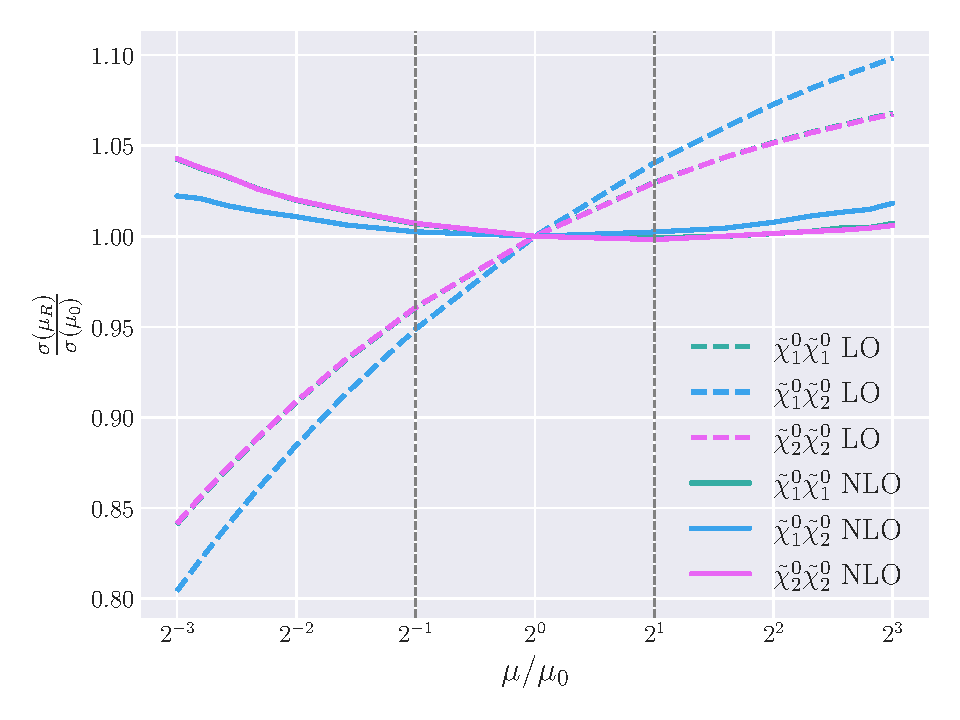
\includegraphics[width=\textwidth]{scaleDependence/scalePlot.pdf}
    \caption{}
  \end{subfigure}
  \caption{Scale dependence of the cross-section for the possible higgsino-like neutralino pairs. The vertical dashed lines indicate the lines for \(\mu_0/2\) and \(2\mu_0\) used to define the scale error.}
  \label{res:fig:scale_dependence}
\end{figure}
\subsection{Scale Dependence}
\label{res:subsec:scale_dependence}
To study the effects of the factorisation and renormalisation scales on the cross-sections, I chose to plot the LO and NLO calculations in the Higgsino scenario with \(\phi_\mu = 0\).
I varied \(\mu_F\) and \(\mu_R\) separately before varying them together, each on the interval \([\frac{1}{8}\mu_0, 8\mu_0]\) where \(\mu_0 = (m_{\tilde\chi^0_i} + m_{\tilde\chi^0_j}) / 2\).
The results are shown in \cref{res:fig:scale_dependence}.
\medskip

In the top left plot of \cref{res:fig:scale_dependence}, we see that the NLO contributions mitigate the factorisation scale dependence on the cross-sections considerably, as we expected from the discussion of renormalised PDFs from \cref{had:subsec:renormalised_pdfs}.
The \(\mu_F\)-dependence is slightly different between the same-type neutralino processes and the different-type neutralino processes, both to LO and NLO, with the overall shape being the same.
There is no obvious explanation for why the different-type neutralino process should be more sensitive on the factorisation scale than same-type processes.

As expected, there is no renormalisation scale dependence in the LO cross-section, as the value of \(\alpha_W\) is kept fixed in our renormalisation scheme discussed in \cref{res:subsec:renormalisation_scheme}, and there is no \(\mu_R\)-dependence in the PDFs or kinematics of the LO contributions.
However, at NLO the results varies up to \(\sim 2.5\%\) up and \(\sim 1.5\%\) down.
This is mostly due to the change in the value of \(\alpha_s\), which is taken at the value of \(\mu_R\) when doing the computations.
It is worth taking note of the fact that the renormalisation scale dependence is inverse to the factorisation scale, in effect reducing the overall scale dependence when they are varied simultaneously in the bottom plot of \cref{res:fig:scale_dependence}.
This should not necessarily be the case generally, but it is noteworthy that it can happen.
The dependence on the renormalisation scale of the different-type neutralino process is different to the same-type processes.

When both scales are varied simultaneously, the overall dependence is somewhat dampened.
Notably, the NLO scale dependence is such that the cross-section is heightened for sufficiently high and low values of \(\mu = \mu_F = \mu_R\).
In practice, this means the theoretical error estimation from the method we use will not have any lower bound below the cross-section value computed with the standard scale \(\mu_0\).
In these cases, I will set the lower bound to be that of the cross-section value \(\sigma(\mu_0)\).
\medskip

Finally, a note on estimating the theoretical error by using the scale dependence.
At LO in Drell-Yan processes, like the ones we have studied in this thesis, \(\alpha_s\) does not enter.
This means scale dependence affecting \(\alpha_s\) will not affect the cross-section to LO, and it will not provide any satisfactory estimation of error resulting from the truncation of the perturbation series in \(\alpha_s\).
To LO, we are agnostic to the strong interaction, seeing only the perturbation series in \(\alpha\), whereas to NLO we `connect' to another, \emph{different} perturbation series in \(\alpha_s\).


\begin{figure}[ht!]
  \centering
  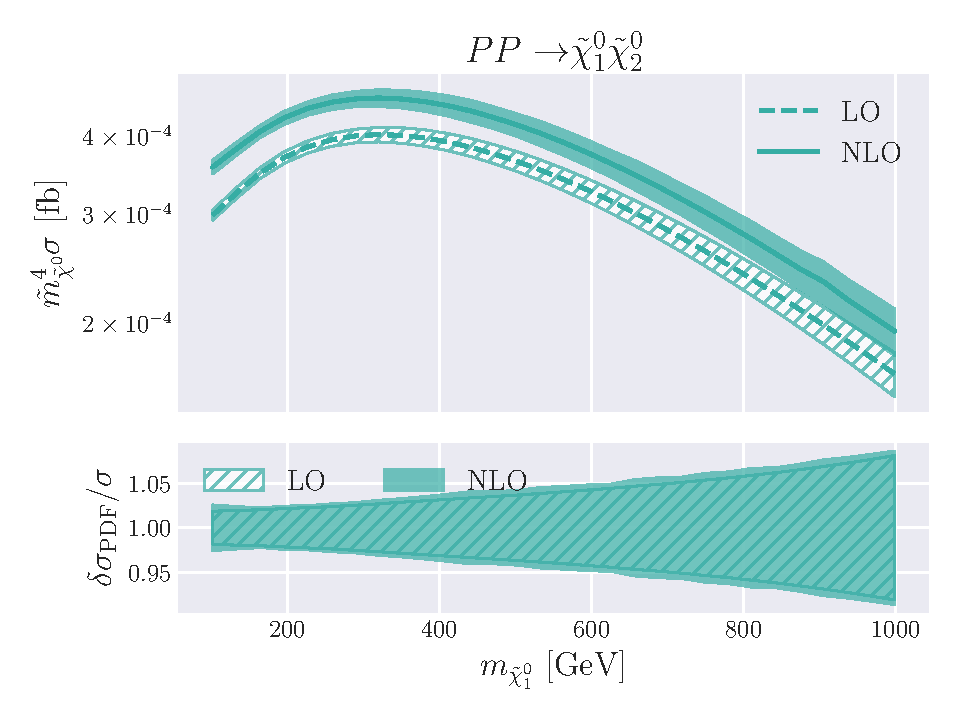
\includegraphics[width=0.85\textwidth]{hinoError/pdfPlot.pdf}
  \caption{Plot of the cross-section for \(\tilde\chi^0_1 \tilde\chi^0_2\) production in the Higgsino scenario with PDF errors added.
    Denoting the mean mass of the final state pair \(m_{\tilde\chi^0} = (m_{\tilde\chi^0_1} + m_{\tilde\chi^0_2}) / 2\), the scaling of the cross-section is given by the dimensionless quantity \(\tilde{m}_{\tilde\chi^0} = m_{\tilde\chi^0} / \operatorname{max}(m_{\tilde\chi^0})\).
    The mass gap between the two neutralinos \(m_{\tilde\chi^0_2} - m_{\tilde\chi^0_1}\) is never greater than \(1.113\) GeV.}
  \label{res:fig:pdf_error}
\end{figure}
\subsection{PDF Errors}
\cref{res:fig:pdf_error} showcases the PDF and \(\alpha_s\) error for pair production of the two lightest neutralinos in the Higgsino scenario to NLO\@ as a function of the Higgs mass parameter \(|\mu|\).
As \(\mu\) is the parameter which governs the higgsino masses, this equates to varying the degenerate mass scale of the two lightest neutralinos in the Higgsino scenario.
The NLO cross-section is again noticeably greater than the LO cross-section, but the overall mass dependence is similar.
A couple of points to make on the PDF errors:
First, it is clear that the errors increase relatively to the cross-section quite linearly with the mass of the produced neutralinos.
This can be explained by the fact that the PDFs are determined to a much lower precision at high values of parton momentum fraction \(x \to 1\)~\cite{PDF4LHCWorkingGroup:2022cjn}.
When the mass of the final state particles increase, more centre-of-mass energy between the colliding partons is necessary to produce the particles, and as such, higher \(x\)-regions of the integral over the PDFs dominate.

The second point to be made is that the PDF uncertainty does not decrease when NLO contributions are taken into account -- to the contrary, the NLO uncertainties are slightly greater than the LO ones.
This could be explained by the fact that the NLO contributions not only depend on the PDFs for the quarks and antiquarks, but also on the PDF of the gluon, as in the quark emission contributions from \cref{had:sec:total_cross_section}.
The PDF of the gluon is not as precisely determined, particularly in low \(x\)-regions, and can thereby add uncertainty to the cross-section.


\begin{figure}[ht!]
  \centering
  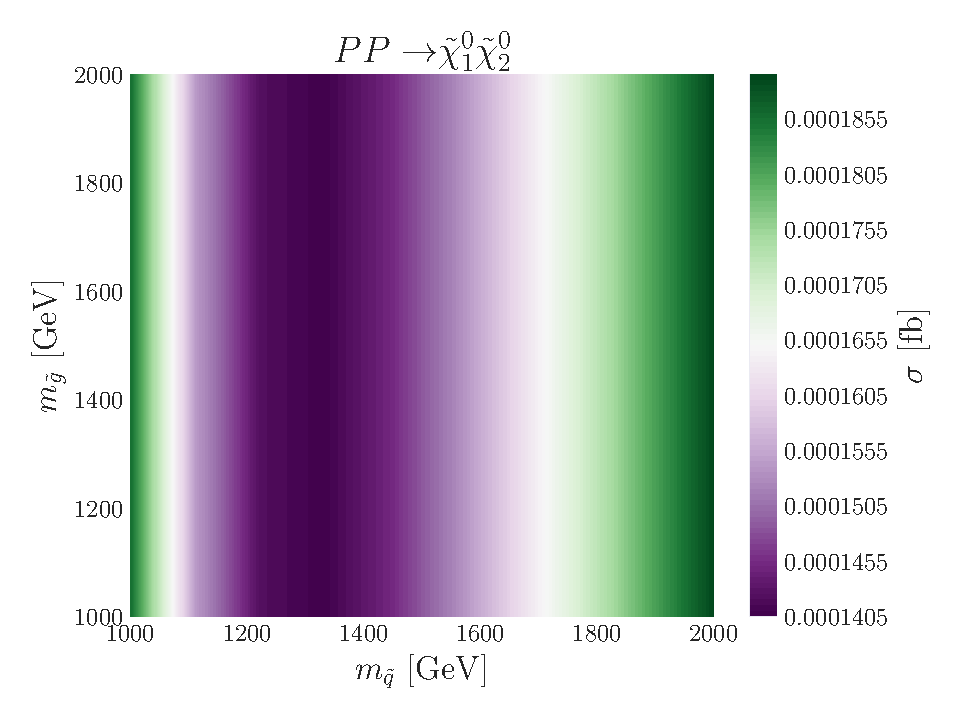
\includegraphics[width=0.85\textwidth]{muCPV/LO.pdf}
  \caption{The scaled cross-section for various neutralino pair production processes as the phase of \(\mu\) is varied in the cSPS1a scenario. Underneath, the relative deviance of the scaled cross-sections as the phase moves away from \(\phi_\mu = 0\) is shown.
  Given the average mass of the final state particles \(m_{\tilde\chi^0} = (m_{\tilde\chi^0_i}+m_{\tilde\chi^0_j})/2\), the scaling is given by \(\tilde{m}_{\tilde\chi^0} = m_{\tilde\chi^0}(\phi_\mu) / m_{\tilde\chi^0}(0)\). This ensures the cross-section for \(\phi_\mu = 0\) is unscaled.
  Scale error is shown with the hatched bands around the lines.}
  \label{res:fig:muCPV}
\end{figure}
\begin{figure}[ht!]
  \centering
  \includegraphics[width=0.85\textwidth]{hinoCPV/NLO.pdf}
  \caption{The scaled cross-section for neutralino pair production of \(\tilde\chi^0_1 \tilde\chi^0_2\) as the phase of \(\mu\) is varied in the Higgsino scenario. Underneath, the relative deviance of the scaled cross-sections as the phase moves away from \(\phi_\mu = 0\) is shown.
  Given the average mass of the final state particles \(m_{\tilde\chi^0} = (m_{\tilde\chi^0_1}+m_{\tilde\chi^0_2})/2\), the scaling is given by \(\tilde{m}_{\tilde\chi^0} = m_{\tilde\chi^0}(\phi_\mu) / m_{\tilde\chi^0}(0)\). This ensures the cross-section for \(\phi_\mu = 0\) is unscaled.
  Scale error is shown with the hatched bands around the lines for the leading order cross-section, and filled bands for the NLO cross-section.}
  \label{res:fig:hinoCPV}
\end{figure}
\section{Exploring CP-Violation}
\label{res:sec:CPV}
To explore the CP violating areas of the MSSM parameter space, I have chosen to focus on the phase of the Higgs mass parameter \(\mu\).
From \cref{res:fig:csps1a_scenario}, we can see that all the neutralino masses are affected by the phase of \(\mu\), and so to mitigate the effect of the differing masses of the final states as \(\phi_\mu\) is varied, I will scale the cross-sections by the average mass of the final state.
I chose to scale using \(\tilde{m}_{\tilde\chi^0}^4\) with a dimensionless scale given by\footnote{Choosing a power of four here is done because the cross-sections roughly go as \(\sigma \sim \frac{1}{m^4}\) where \(m\) is the average mass of the final state particles.}
\begin{equation}
  \tilde{m}_{\tilde\chi^0}(\phi_\mu) = \frac{m_{\tilde\chi^0}(\phi_\mu)}{m_{\tilde\chi^0}(0)},
\end{equation}
where \(m_{\tilde\chi^0}(\phi_\mu)\) is the average final state mass given by
\begin{equation}
  m_{\tilde{\chi}^0}(\phi_\mu) = \frac{m_{\tilde\chi^0_i}(\phi_\mu) + m_{\tilde\chi^0_j}(\phi_\mu)}{2}.
\end{equation}
Scale error is included in the plots in this section, calculated by varying \(\mu_F\) and \(\mu_R\) together.

\subsection{cSPS1a scenario}
In the cSPS1a scenario, I chose to examine four different neutralino pairs:
Same pair production of the bino-like \(\tilde\chi^0_1\) and wino-like \(\tilde\chi^0_2\), pair production mixing wino-like and higgsino-like states \(\tilde\chi^0_2\) and \(\tilde\chi^0_3\), and pair production of the two different higgsino-like states \(\tilde\chi^0_3\) and \(\tilde\chi^0_4\).
The results are shown in \cref{res:fig:muCPV}.

Greatest relative effect is seen in the cross-sections for the \(\tilde\chi^0_2\) pair and \(\tilde\chi^0_2 \tilde\chi^0_3\) pair.
This is not unnatural, as variation in the mass of \(\tilde\chi^0_2\) is greatest from \cref{res:fig:csps1a_scenario}, relative to the original mass at \(\phi_\mu = 0\).
Perhaps more surprisingly, the cross-section for \(\tilde\chi^0_2\) pair production is greater than that of the lightest neutralino \(\tilde\chi^0_1\), by about a factor of two.
It is worth noting that all cross-sections see the greatest difference in value when \(\phi_\mu = \pi\), corresponding with flipping the sign of \(|\mu|\).
Scale dependence seems largely unaffected by \(\phi_\mu\).


\subsection{Higgsino Scenario}
To explore the effect of the phase of \(\mu\) on the NLO corrections to the cross-sections, I return to the Higgsino scenario, with \(|\mu| = 100\) GeV.
Computing just the process of pair production of the two different higgsino states in this scenario, the results are shown in \cref{res:fig:hinoCPV}.

As we have seen earlier, the NLO corrections boost the cross-section quite significantly from the LO result, far exceeding the scale error, as discussed in \cref{res:subsec:scale_dependence}.
I note that the scale error decreases by quite a bit in the NLO cross-section, which can be due to the cancellation between \(\mu_F\) and \(\mu_R\) errors, again discussed in \cref{res:subsec:scale_dependence}.
Furthermore, the \(\phi_\mu\) dependence is mitigated as the NLO contributions are taken into account, suggesting that the NLO contributions are not as sensitive to \(\phi_\mu\) as the LO contribution, at least in the scenario at hand.
This seems reasonable, as the NLO contributions come from strongly interacting particles not directly tied to the Higgs mass parameter \(\mu\).
The maximal relative deviance from the \(\phi_\mu = 0\) cross-sections is near the regions of maximal complex phase of \(\mu\), contrary to what we see in \cref{res:fig:muCPV}.
In fact, the cross-section seems invariant under a phase shift of \(\phi_\mu \to \phi_\mu + \pi\), corresponding to multiplying \(\mu\) by \(-1\).




\begin{figure}[ht!]
  \centering
  \includegraphics[width=0.85\textwidth]{hinoMassCPV/NLO.pdf}
  \caption{Scaled NLO cross-section results for pair production of the two lightest neutralinos in the Higgsino scenario as both \(|\mu|\) and \(\phi_\mu\) are varied.
  Given the average mass of the final state particles \(m_{\tilde\chi^0} = (m_{\tilde\chi^0_1}+m_{\tilde\chi^0_2})/2\), the scaling is given by \(\tilde{m}_{\tilde\chi^0} = m_{\tilde\chi^0}(\phi_\mu) / m_{\tilde\chi^0}(0)\). This ensures the cross-section for \(\phi_\mu = 0\) is unscaled.}
  \label{res:fig:hinoMassCPV}
\end{figure}
\begin{figure}[ht!]
  \centering
  \begin{subfigure}{0.49\textwidth}
    \centering
    \includegraphics[width=\textwidth]{squarkGluinoMass/hinoNLO.pdf}
    % 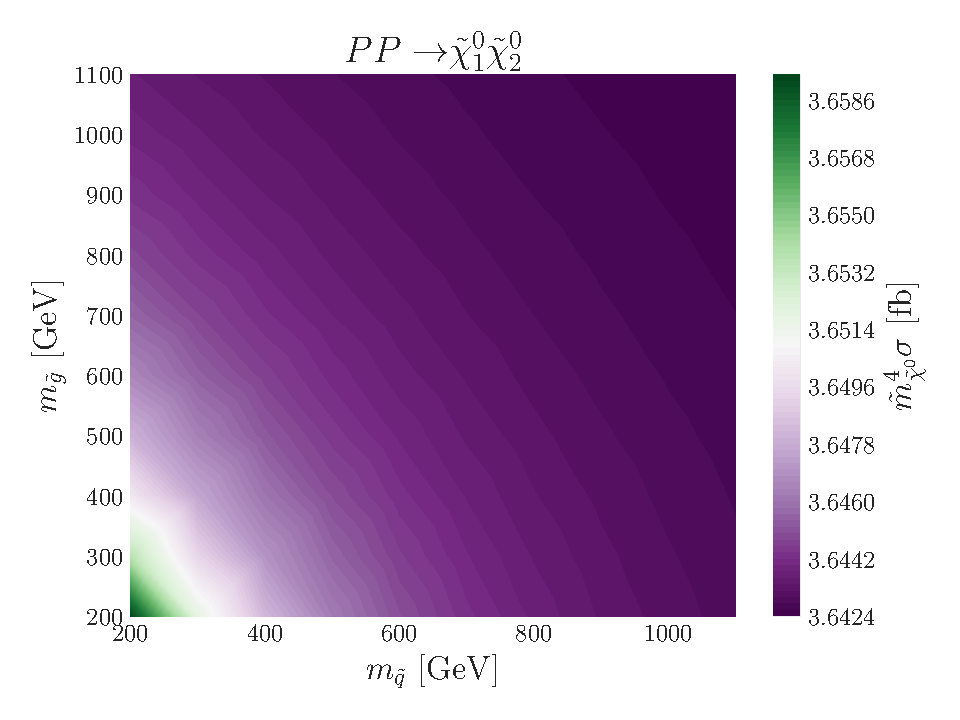
\includegraphics[width=\textwidth]{squarkGluinoMass/hinoNLO_corrected.pdf}
    \caption{}
  \end{subfigure}
  \begin{subfigure}{0.49\textwidth}
    \centering
    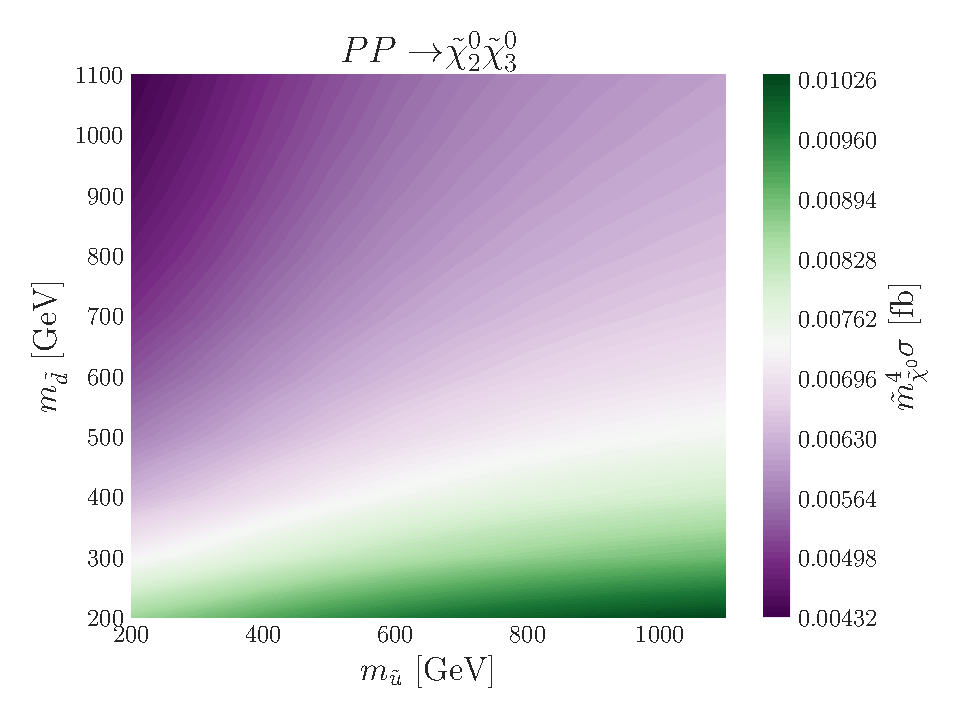
\includegraphics[width=\textwidth]{squarkGluinoMass/csps1a_2325.pdf}
    \caption{}
  \end{subfigure}
  \caption{\textbf{(a)} Depicts the cross-section for pair production of the two lightest neutralinos to NLO in the simplified Higgsino scenario as the common squark mass and the gluino mass is varied separately.\\
    \textbf{(b)} Depicts the cross-section for neutralino pair production in the cSPS1a scenario as the common up-type and down-type squark masses are varied separately.}
  \label{res:fig:squarkGluinoMass}
\end{figure}
\section{Exploring Other Parameters}
So far, we have mainly investigated the Higgs mass parameter \(\mu\) and its phase \(\phi_\mu\).
In this section, I  will explore variation of these two parameter simultaneously, and dependence on the squark and gluino masses.
The squark mass is of particular interest, as it is the mediator of the interaction for producing gaugino-like neutralinos.
I also note that all the plots are generated from a ten by ten grid of cross-section values with simple triangulation interpolation applied for visualisation.
In general, this is not good practice, however in our case I am simply trying to present an idea of the parameter dependence, rather than rigorous analysis in comparison to experiments.


\subsection{Varying Higgsino Masses and CP-Violation}
The magnitude and phase of the Higgs mass parameter \(\mu\) were varied together in the Higgsino scenario in \cref{res:fig:hinoMassCPV} to NLO\@.
The cross-sections were scaled according to the same prescription as in \cref{res:sec:CPV}.
Along the \(x\)-axis, the lightest neutralino mass is shown, but seeing as the two lightest neutralinos are quite mass degenerate in this scenario, the next-to-lightest neutralino mass is not much higher.

The dependence on the higgsino masses seem to have a shape overall similar to the results with \(\phi_\mu = 0\) used in \cref{res:fig:pdf_error}.
In fact, this dependence seems to dominate over the effect of the complex phase of \(\mu\).


\subsection{Varying Squark and Gluino Masses}
To vary the squark and gluino masses, I will use slightly different scenarios to the ones I have used thus far, although they will be based on the cSPS1a and Higgsino scenarios.
Particularly, I will not generate the particle spectra from MSSM Lagrangian parameters, but rather use the standard cSPS1a scenario with \(\phi_\mu = 0\) (which reproduces the SPS1a scenario), and the simplified higgsino scenario from the comparison to SXWG from \cref{res:sec:comparison}.
When varying this cSPS1a scenario, I will keep all parameters fixed (including the squark mixing angles), while setting all up-type squark masses and down-type squark masses are set to be degenerate respectively.
In the simplified higgsino scenario, no mixing between the chiral squark states is assumed, and all the squark masses are set to be the same.

The squark mass \(m_{\tilde{q}}\) and gluino mass \(m_{\tilde{g}}\) will then be varied separately in these simplified, unnatural scenarios.\footnote{These are unnatural in the sense that the parameters are not cohesive, being derived from a single, physical Lagrangian.}
\medskip

The results can be seen in \cref{res:fig:squarkGluinoMass}.
In the left plot, we can see the simplified Higgsino scenario to NLO, showing that even though no squark or gluino parameters affect the LO cross-section, there is still quite significant sensitivity to them at NLO\@.
Particularly for low squark and gluino masses, the cross-section is enriched quite dramatically as compared to the higher values for these masses.
The squark mass seems especially important when computing these effects.
\medskip

In the right plot, we can see the LO production of the wino-like next-to-lightest neutralino together with the higgsino-like next-to-heaviest neutralino in the cSPS1a scenario.
This cross-section is suppressed, as the two different neutralino types do not share a common channel.
However, the cross-section is quite dependent on the squark masses, being enriched for low down-type squark masses and high up-type squark masses.
This suggests that the up-type squark mediated contributions interfere negatively with the \(Z\)-boson mediated and down-type squark mediated contributions, as turning it off seems to increase the contribution.

In the right plot, we can see the production of bino- and wino-like lightest two neutralinos of the cSPS1a scenario to LO\@.
Their production is mediated by the squark, so it is natural to see that the dependence on the squark masses governs the overall cross-section.
In fact, the impact of the gluino

\ifSubfilesClassLoaded{%
  \bibliography{references}{}
  \bibliographystyle{style/JHEP}
}{}

\end{document}
